\vspace{-20pt}
\section{Bugs}
\doom{} is known for its stability partly thanks to a development process using seven compilers and systems. Nonetheless it shipped with a few bugs.








\subsection{Flawed collision detection}
One rare collision detection bug was first brought to light (and subsequently explained in depth) by Colin "cph" Phipps in his article "Shooting Through Things".\\
\par
\fq{A monster is getting too close for comfort. You shoot at it, and miss. If you are unlucky, the monster kills you. But you were so sure that you were pointing right into the monster, that so close as you were you couldn't have missed. Perhaps it was the chaingun playing up, shooting all the bullets off to one side. Perhaps the game was written by a bunch of losers who failed their high-school geometry. Or perhaps, in the heat of the moment, you really did miss; nobody's perfect.\\
\par
Well I have good news. You can blame your tools.}{Colin Phipps}\\
\par
Some enemies can be really big, almost ten times bigger than the player (16 units), such as in the case of the Spider Mastermind (128 units). As we saw on page \pageref{E1M1_blockmap}, \doom{} uses blockmaps to speed up detection of intersections with things and walls. If a thing is on the edge of block and the player is a bit unlucky, what should have been a hit can end up as a miss.

\fullimage{beasts_sizes.png}
\vspace{-1cm}
\fullimage{beasts_sizes2.png}


\rawdrawing{collision_miss}
\par
It is possible to miss a SpiderDemon in a hallway. In the single room map above, the green player on the left is firing at a red enemy 128 units wide on the right (probably a SpiderDemon). The blue grid shows the blockmap's alignment.\\
\par
 The line of the bullet and the radius of the monster clearly overlap. This should be a hit. But only the content of blockmaps \cw{0}, \cw{1} and \cw{2} will be checked, resulting in tests with walls \cw{D}, \cw{A} and \cw{B}. Since the enemy is in block \cw{5} and the bullet doesn't cross it, the hit is not registered.\\
 \par
 This bug is not limited to very large monsters. It can happen with any enemy depending on how close they are to the player and how the blockmaps align.







\subsection{Slime trail}
A slime trail happens when there is a horizontal screen space gap between two walls. Visplanes "leak" between the space, resulting in graphical glitches. This was a known issue during development that was never fixed due to deadlines and the fact they only rarely occurred. John Carmack mentioned it when the \cw{doombsp} source code was released.\\
\par
\fq{There IS a bug in here that can cause up to a four pixel wide column to be drawn out of order, causing a more distant floor and ceiling plane to stream farther forward than it should.  You can sometimes see this on E1M1 looking towards the imp up on the ledge at the entrance to the zig zag room.  A few pixel wide column of slime streams down to the right of the walkway.  It takes a bit of fidgeting with the mouse to find the spot.  If someone out there tracks it down, let me know...
}{John Carmack}\\
\par


\fullimage{slime_trail.png}

The issue can actually be far wider than four pixels if one knows where to look.\\
\par
\fullimage{big_slime_trail.png}
\par
This particular instance of slime trail is the result of the engine's visplane inference system combined with the limited precision of integers when a map is sliced up by via \cw{doombsp}.\\
\par
 Once again, let's take an example. The two previous screenshots were taken in the very first map of the game, E1M1, in a zigzag section surrounded by toxic green liquid. At first glance, there is nothing unusual here but when we take a look at how it was sliced during binary partitioning, an interesting special case appears.\\
\par
Line \cw{A} was selected as a splitter. As it crosses lines \cw{B} and \cw{G}, two segments are created as \cw{B1}, \cw{B2}, \cw{G1}, and \cw{G2}. The new vertices created are in red. Things are less clear for lines C and E (or is it F ?). We need to look closer. \\
\par
If we zoom in on vertex \cw{3}, we see the splitter crossed \cw{F} between integer coordinates. Since map vertex coordinates are stored as integers, a split is impossible. The error is small, so \cw{doombsp} treats the vertex as if it was exactly on the splitting line.

\begin{minipage}{0.47\textwidth}
\rawscaleddrawing{1}{E1M1_slimetrail}
\end{minipage}
\hspace{4mm}
\begin{minipage}{0.47\textwidth}
\rawscaleddrawing{1}{E1M1_slimetrail_split}
\end{minipage} 
\par
\vspace{1mm}
\rawdrawing{E1M1_slimetrail_zoom}
\par



\fullimage{leak_opposite.png}
\par
\begin{wrapfigure}[22]{r}{0.45\textwidth}
\centering
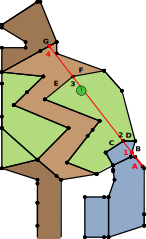
\includegraphics[width=.45\textwidth]{drawings/E1M1_slimetrail_split2.pdf}
\end{wrapfigure}
Let's position the player along the same split line we just studied, but facing the opposite direction (the scene is simpler with fewer walls). The player is very close to segments \cw{E} and \cw{F} (which is where the rendering error is). Further in the background are segments \cw{G1} and \cw{G2} where line \cw{G} was split.\\
\par
The frame starts with a blank canvas. Portal \cw{E} is rendered first. It has no upper or middle texture but it does have a lower texture that is drawn (marked with a green overlay on page \pageref{leak_opposite_explained.png}). As the lower texture is rendered, the screen space below is inferred to be a floor visplane \cw{E-VP} (shown with a pink overlay). The engine then continues down the BSP and renders \cw{G1}.\\
\par

 \cw{G1}'s lower texture is rendered (in red). Everything below that is inferred to be a floor and therefore visplane \cw{G1-VP} is created. Notice that the visplane goes all the way to the bottom of the screen which is is a rendering bug. Had the BSP been split properly, \cw{F1} would have been rendered before \cw{G1} and stopped the visplane from flooding in screenspace improperly.\\
\par
 

\fullimage{leak_opposite_explained.png}\\
\label{leak_opposite_explained.png}
\par
From there, the damage is done. The engine renders the other side of the BSP and hits \cw{F} which is clipped against the vertical boundary set by \cw{G1} and then drawn (in blue). The space below \cw{F} is inferred to be floor and visplane \cw{F-VP} (turquoise) is generated\footnote{The engine actually merges \cw{E-VP} and \cw{F-VP} but let's discard it for the sake of simplicity.}.


\section{Barrel suicide}
\doom{} monsters are capable of fighting against each other. If friendly fire was to occur during combat, the damaged monster will automatically attempt to retaliate instead of attacking the player. This is called monster infighting.\\
\par
There is an amusing special case of infighting which involves exploding barrels. When a barrel is damaged, the engine "memorizes" which entity was responsible for it. When the barrel actually explodes the source of the damage is passed to all damaged entities so they can retaliate.\\
\par
What can happen is that a monster triggers a barrel to explode and gets injured by the blast in the process. In this occurrence, monsters with a melee attack (Cacodemon, Imp, Hellknight) will "tear themselves apart" while those only capable of range attack (former humans) will go nuts and fire blindly at random, possibly triggering further monster infighting.